\label{ch:results_jena}

\subsection{Results}

\subsubsection*{Visitation Rates}			

In total, I made 385 observations, each representing pollinator activity records for 15min in a 80cm x 80cm plot. In total, I analyzed data from 96,25h of observation on 246.4m$^{2}$.

\textit{Onobrychis viciifolia} was the most attractive plant with a maximum of 318 visits in one observation. The per-flower visitation rate varied strongly with the attractiveness of the focal species. Per observation, I recorded 1.4 $\pm$ 1.8 (mean $\pm$ SD) visits per flower with a maximum of 10.7 visits per flower (again \textit{Onobrychis viciifolia}) and 31 observation with no visit at all to the focal species. The per-flower visitation rate was significantly different between the two very attractive species \textit{Geranium pratense} and \textit{Onobrychis viciifolia} and the three less attractive species  \textit{Trifolium pratense}, \textit{Lotus corniculatus} and \textit{Lathyrus pratensis} (\textit{P} $\leq$ 0.001, tab.~\ref{tab:VR_spec}). The subplots contained 3 $\pm$ 1.2 (mean $\pm$ SD) flowering species including the focal species, the species richness was higher at the plot level with 8 $\pm$ 2.4 (mean $\pm$ SD) flowering species.

\begin{table}[!htbp] %VR species
	\centering
	\caption{Per-flower visitation rates (mean $\pm$ SD) for the focal flower species per 15 minute observation. \textit{Geranium pratense} and \textit{Onobrychis viciifolia} are significantly different from the other three species (pairwise t-test, \textit{p} $<$ 0.001) . Within the two groups, there is no significant difference between the species. }
	\begin{tabular}{l l l l l}
		\toprule
		\textbf {Short} & \textbf{Species} & \textbf{Family} &\textbf{Visitation Rate (Mean)} & \textbf{ $\pm$ SD} \\
		\midrule
		Ger  & \textit{Geranium pratense} & Geraniaceae & 3.05 & 1.5 \\ %109
		Lat  & \textit{Lathyrus pratensis} & Fabaceae & 0.57 & 0.53 \\ %83
		Lot  & \textit{Lotus corniculatus} & Fabaceae & 0.30 & 0.36 \\  % 77
		Ono  & \textit{Onobrychis viciifolia} & Fabaceae & 3.60  &  2.5 \\ % 37
		TP   & \textit{Trifolium pratense} & Fabaceae & 0.16 & 0.23 \\ % 79
		\bottomrule
	\end{tabular}%
	\label{tab:VR_spec}
\end{table}%


\subsubsection*{Frequency Dependence}			
Floral cover and species richness had both individually and in the interaction term with frequency no effect on the visitation rate and were removed from the model (Cover: F$_{df\shorteq1}$ = 1.17, \textit{P} = 0.28; Species Richness: F$ _{df\shorteq1} $ = 1.15, \textit{P} = 0.29). 
%Freq:Cover 0.446 //Freq:SR 0.426

The linear mixed effect model showed an effect of species and frequency individually and with interactions on the per-flower visitation rate (Species: F$_{df\shorteq4}$ = 141.13, \textit{P} $\leq$ 0.0001; Frequency: F$_{df\shorteq1}$ = 18.29, \textit{P} $\leq$ 0.0001; Species x Frequency F$_{ df\shorteq4}$ = 5.2, \textit{P} $\leq$ 0.001, tab.~\ref{tab:anova}). Interestingly, frequency contributed also as quadratic and cubic term with its interactions to species explanatory power to the model, giving the relationship a non-linear character (Tab.~\ref{tab:anova}). Figure~\ref{fig:LME} showed the cubic relationship of four focal species and the summed data and a quadratic relationship for \textit{Lathyrus pratensis}. The cubic curve is defined by a strong increase for frequencies below 20\% followed by a minimum between 50 and 80\% depending on the species before raising again with increasing dominance of the focal species. However, the visitation rate of \textit{Lathyrus pratensis} showed a maximum at 60\% frequency and decreases afterwards. 

\begin{figure} [!th] %LME
	\centering
	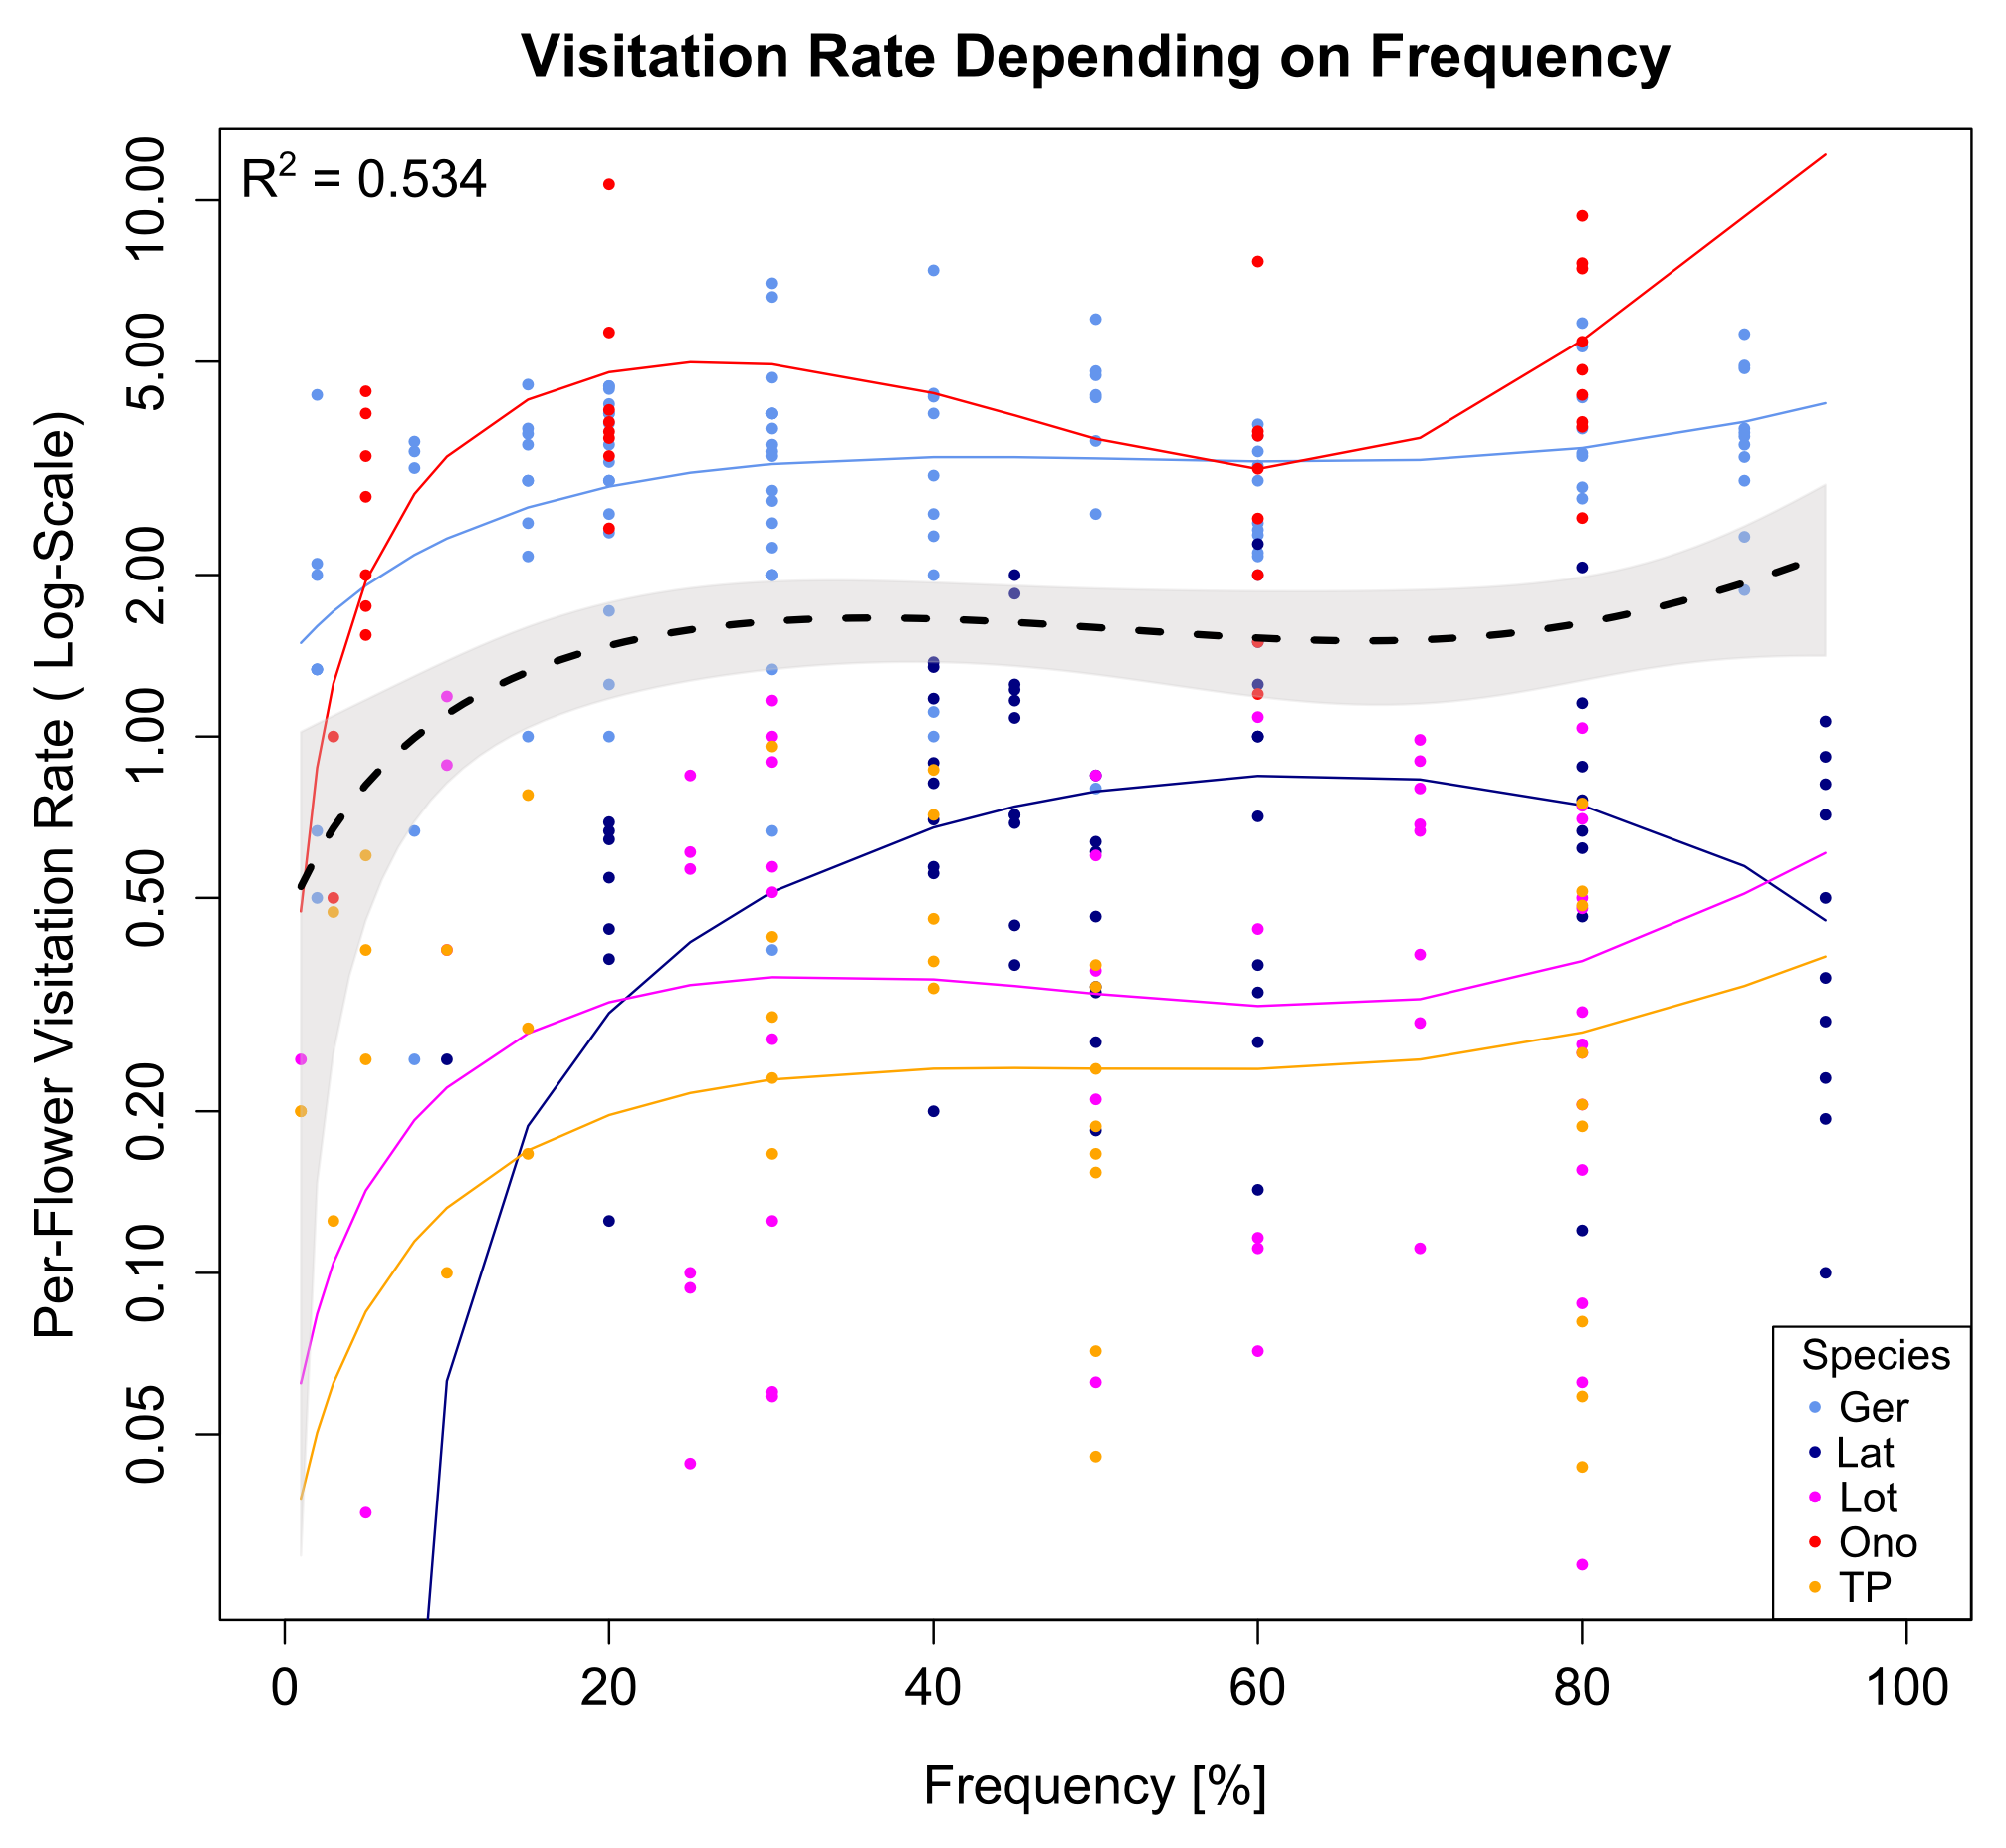
\includegraphics[width=14cm]{Images/LME}
	\caption{Per-flower visitation rates of the five focal species over different frequencies. Each point represents one observation of 15 minutes. The y-axis is plotted on a log scale due to the variance in attractiveness of the focal species. The linear mixed effect model with patch nested in plot as random factor show a cubic frequency dependence for all species but \textit{Lathyrus pratensis}. Floral cover and species richness were dropped as explanatory variables in the model selection process. R$^{2}$ was calculated with the "r.squaredGLMM"-function of the MuMIn-Package \citep{MuMIn}}
	\label{fig:LME}
\end{figure}

\begin{table} [!htbp] %results lme
	\centering
	\caption{Results of the linear mixed effect model with per-flower visitation rate as explanatory variable. Floral cover and species richness and its interactions with frequency were not relevant predictors for the model and therefore removed in the model selection process (denDF = 191, R$^{2}$ = 0.53, n = 385)}
	\begin{tabular} { l l c c c}
		\toprule
		\textbf{Response Variable} & \textbf{Explanatory Variables} & \textbf{Df} & \textbf{F-value} & \textbf{\textit{P}} \\
		\midrule
		Per-flower visitation rate   & Species & $4$ & $130.9$ & $<0.0001$\\
		& Frequency 			&  $1$ & $49.3$ & $<0.0001$ \\
		& Frequency$^{2}$ 		&  $1$ & $13.2$ & $0.0026$ \\
		& Frequency$^{3}$ 		&  $1$ & $ 5.8$ &  $0.8145$ \\
		& Frequency x Species &  $4$ & $ 5.2$ &  $0.0005$ \\
		& Frequency$^{2}$ x Species & $4$ & $3.4$ & $0.0097$\\
		& Frequency$^{3}$ x Species & $4$ & $3.4$ & $0.0101$\\
		\bottomrule
	\end{tabular}
	\label{tab:anova}
\end{table}
